\section{问题一：典型风光场景下运行指标分析}

\subsection{模型建立}

问题一的求解思路为：首先根据附件数据计算各时段的实际功率，然后通过功率平衡方程确定购售电功率，最后计算各项能量指标和绿电直连指标。求解流程如图\ref{fig:flow_q1}所示。

\begin{figure}[H]
\centering
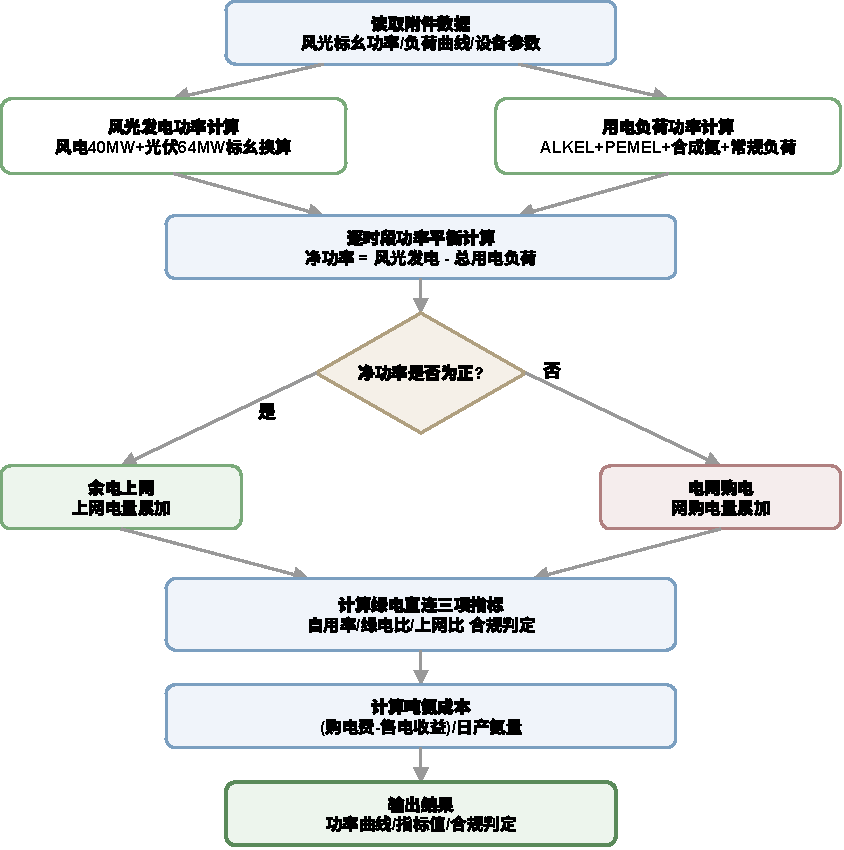
\includegraphics[width=0.85\textwidth,height=0.38\textheight,keepaspectratio]{../figures/fig_flow_q1.pdf}
\caption{问题一求解流程图}\label{fig:flow_q1}
\end{figure}

在电解槽与合成氨装置满负荷连续运行条件下，园区每时段的制氢氨负荷功率为常数：
\begin{equation}
P_{\text{H2NH3}} = P_{\text{ALKEL}}^{\text{rated}} + P_{\text{PEMEL}}^{\text{rated}} + P_{\text{NH3}}^{\text{rated}} = 10 + 10 + 0.75 = 20.75 \text{ MW}
\end{equation}

园区总用电负荷功率为制氢氨负荷与常规电负荷之和：
\begin{equation}
P_{\text{total}}(t) = P_{\text{H2NH3}} + P_{\text{load}}(t), \quad t = 1, 2, \ldots, 24
\end{equation}

根据功率平衡原则，定义净功率为新能源发电与总负荷之差：
\begin{equation}
P_{\text{net}}(t) = P_{\text{wind}}(t) + P_{\text{pv}}(t) - P_{\text{total}}(t)
\end{equation}

由互补约束$P_{\text{buy}}(t) \cdot P_{\text{sell}}(t) = 0$，购售电功率由净功率的正负确定：
\begin{equation}
P_{\text{sell}}(t) = \max(P_{\text{net}}(t), 0), \quad P_{\text{buy}}(t) = \max(-P_{\text{net}}(t), 0)
\end{equation}

\subsection{能量指标计算}

各能量指标通过对功率进行时间积分得到（时段长度$\Delta t = 1$~h）：
\begin{equation}
E_{\text{use}} = \sum_{t=1}^{24} P_{\text{total}}(t) \cdot \Delta t, \quad E_{\text{RE}} = \sum_{t=1}^{24} [P_{\text{wind}}(t) + P_{\text{pv}}(t)] \cdot \Delta t
\end{equation}
\begin{equation}
E_{\text{buy}} = \sum_{t=1}^{24} P_{\text{buy}}(t) \cdot \Delta t, \quad E_{\text{sell}} = \sum_{t=1}^{24} P_{\text{sell}}(t) \cdot \Delta t
\end{equation}

绿电直连三项指标按题目给定公式计算：
\begin{equation}
r_1 = \frac{E_{\text{use}} - E_{\text{sell}} - E_{\text{buy}}}{E_{\text{RE}}} \times 100\%
\end{equation}
\begin{equation}
r_2 = \frac{E_{\text{RE}} - E_{\text{sell}}}{E_{\text{use}}} \times 100\%
\end{equation}
\begin{equation}
r_3 = \frac{E_{\text{sell}}}{E_{\text{RE}}} \times 100\%
\end{equation}

\subsection{吨氨成本模型}

吨氨成本综合考虑购电成本、售电收入、新能源度电成本、制氢运维成本和设备折旧：
\begin{equation}
C_{\text{ton}} = \frac{C_{\text{buy}} - R_{\text{sell}} + C_{\text{RE}} + C_{\text{OM}} + C_{\text{dep}}}{Q_{\text{NH3}}}
\end{equation}

其中购电成本$C_{\text{buy}} = \sum_{t=1}^{24} \lambda_{\text{buy}}(t) \cdot P_{\text{buy}}(t) \cdot 1000$（元），售电收入$R_{\text{sell}} = \sum_{t=1}^{24} 0.3779 \cdot P_{\text{sell}}(t) \cdot 1000$（元），新能源度电成本$C_{\text{RE}} = 150 \cdot E_{\text{wind}} + 120 \cdot E_{\text{pv}}$（元），制氢运维成本$C_{\text{OM}} = (100 \cdot E_{\text{ALKEL}} + 150 \cdot E_{\text{PEMEL}} + 2 \cdot E_{\text{NH3}})$（元），合成氨装置日折旧$C_{\text{dep}} = 18000000 / (30 \times 365) = 1643.84$元/日。

\subsection{计算结果}

\subsubsection{功率平衡曲线}

将附件1的常规电负荷标幺功率乘以峰值6~MW，附件2的风电、光伏标幺功率分别乘以装机容量40~MW和64~MW，得到各时段实际功率值。典型日功率平衡曲线如图\ref{fig:q1_power_balance}所示。

\begin{figure}[H]
\centering
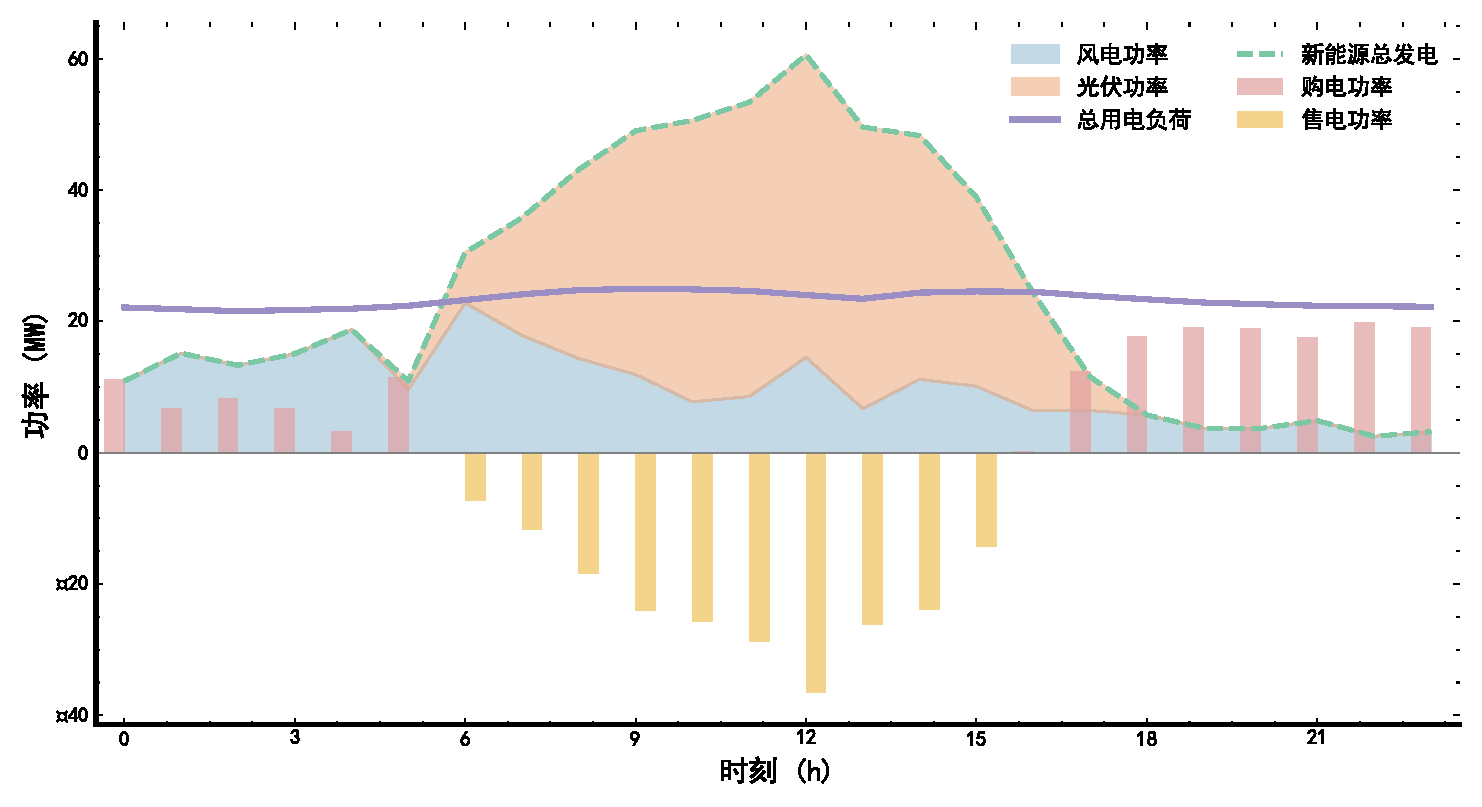
\includegraphics[width=0.95\textwidth]{../figures/fig_q1_power_balance.pdf}
\caption{典型日功率平衡曲线}\label{fig:q1_power_balance}
\end{figure}

由图\ref{fig:q1_power_balance}可以观察到明显的时序不匹配特征：风光发电集中在7:00--17:00时段，峰值出现在13:00左右（约60.6~MW），而制氢氨负荷全天恒定运行（20.75~MW）。在白天高峰时段，新能源发电远超负荷需求，最大余电功率达36.59~MW（13:00时段）；而在夜间（18:00--次日6:00），光伏出力为零，仅靠风电难以满足负荷需求，最大购电功率达19.81~MW（23:00时段）。这种时序错配是导致绿电直连指标不达标的根本原因。

\subsubsection{能量指标与绿电直连指标}

计算得到的各项能量指标和绿电直连指标如表\ref{tab:q1_energy}所示。

\begin{table}[H]
\centering
\caption{问题一能量指标与绿电直连指标}\label{tab:q1_energy}
\begin{tabular}{lccl}
\toprule
指标 & 数值 & 单位 & 达标情况 \\
\midrule
风电日发电量 $E_{\text{wind}}$ & 245.05 & MWh & --- \\
光伏日发电量 $E_{\text{pv}}$ & 358.40 & MWh & --- \\
新能源总发电量 $E_{\text{RE}}$ & 603.45 & MWh & --- \\
园区总用电量 $E_{\text{use}}$ & 558.72 & MWh & --- \\
网购电量 $E_{\text{buy}}$ & 172.04 & MWh & --- \\
上网电量 $E_{\text{sell}}$ & 216.77 & MWh & --- \\
\midrule
自发自用比例 $r_1$ & 28.16 & \% & 不满足（要求$>$60\%） \\
绿电比例 $r_2$ & 69.21 & \% & 满足（要求$>$30\%） \\
上网电量比例 $r_3$ & 35.92 & \% & 不满足（要求$<$20\%） \\
\midrule
吨氨成本 $C_{\text{ton}}$ & 4368.00 & 元/吨 & --- \\
\bottomrule
\end{tabular}
\end{table}

绿电直连指标的实际值与政策要求值的对比如图\ref{fig:q1_indicators}所示。

\begin{figure}[H]
\centering
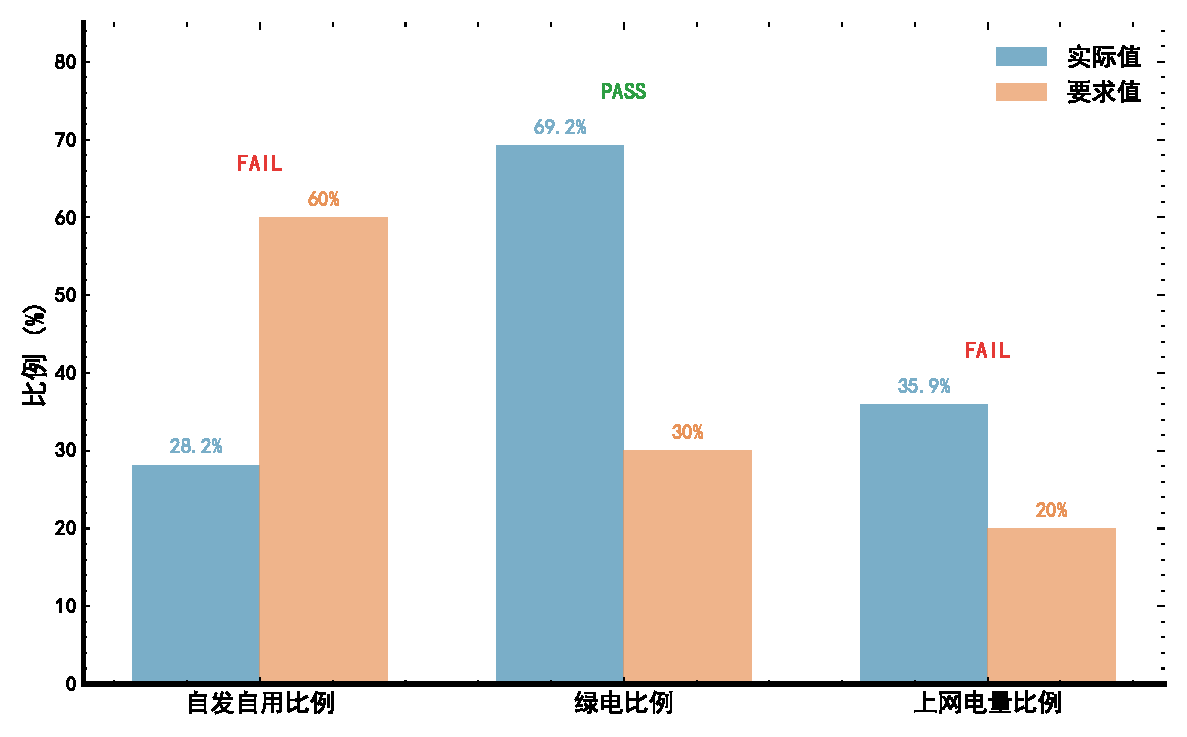
\includegraphics[width=0.85\textwidth]{../figures/fig_q1_indicators.pdf}
\caption{绿电直连指标实际值与要求值对比}\label{fig:q1_indicators}
\end{figure}

\subsection{指标不满足原因分析}

三项绿电直连指标中，仅$r_2 = 69.21\%$满足要求（$>30\%$），$r_1$和$r_3$均不达标。分析原因如下：

$r_1 = 28.16\%$远低于60\%的要求，其物理含义为新能源自发自用电量占总发电量的比例。由于光伏仅在6:00--18:00有出力，而制氢氨负荷全天24小时均匀运行，白天大量风光电力无法被负荷消纳而上网，导致自发自用比例偏低。从能量平衡角度看，自发自用电量 = $E_{\text{use}} - E_{\text{sell}} - E_{\text{buy}}$ = 558.72 - 216.77 - 172.04 = 169.91~MWh，仅占新能源总发电量603.45~MWh的28.16\%。

$r_3 = 35.92\%$远高于20\%的上限要求，表明上网电量过多。上网电量216.77~MWh占新能源总发电量的35.92\%，主要来源于白天7:00--16:00时段风光出力高峰期间的余电。这一问题的本质是园区缺乏足够的柔性负荷或储能手段来消纳白天的富余电力。

上述分析表明，在满负荷连续运行模式下，风光出力与负荷需求的时序错配是导致绿电直连指标不达标的根本原因。问题二和问题三通过调节制氢氨负荷的运行时段和功率水平来改善这一问题。
